95. \begin{figure}[ht!]
\center{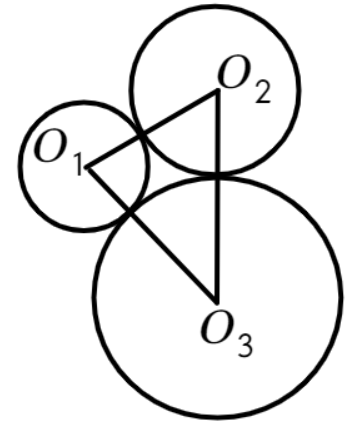
\includegraphics[scale=0.35]{g8-95.png}}
\end{figure}\\
Точки касания окружностей лежат на одной прямой с их центрами, поэтому $O_1O_2=2+4=6,\ O_1O_3=2+6=8,\ O_2O_3=4+6=10.$ Так как $6^2+8^2=10^2,$ по обратной теореме Пифагора треугольник $O_1O_2O_3$ является прямоугольным. Посчитаем его площадь двумя способами. С одной стороны, она равна $6\cdot8:2=24,$ а с другой $rp=r\cdot\cfrac{6+8+10}{2}=12r.$ Значит, $r=24:12=2.$
ewpage
oindent
